\documentclass[bluish,slideColor,colorBG,pdf]{prosper}
\hypersetup{pdfpagemode=FullScreen}
\usepackage{graphicx}
\usepackage{epsfig}
\def\baselinestretch{1.0}
\setlength{\topmargin}{-60pt}
\setlength{\textheight}{460pt}
\setlength{\oddsidemargin}{0pt}
\setlength{\evensidemargin}{0pt}
\setlength{\textwidth}{660pt}
\setlength{\footskip}{0pt}
\parindent 0.3in
\hyphenpenalty=10000
\tolerance=10000
\pagestyle{empty}

\def\Prob{{\rm Prob\;}}
\def\prob{{\rm \;Prob\;}}


\author{February 2017}
\title{Genome 562}
\institution{Week 7}

\begin{document}

\maketitle

\begin{slide}[Replace]{Julian Huxley (1887-1975) }
\bigskip

\begin{center}
\begin{tabular}{c c}

\includegraphics[height=2.0in]{Huxley1922.ps} &
\includegraphics[height=2.0in]{huxleyj.ps}\\
 & \\
Oxford University, 1922 & about 1960 
\end{tabular}
\end{center}
\end{slide}

\begin{slide}[Replace]{Sewall Wright (1889-1988) }

\centerline{\includegraphics[width=1.5in]{wright.ps}}
\medskip

\centerline{At the University of Chicago, 1929}

\end{slide}

\begin{slide}[Replace]{}

\centerline{\includegraphics[width=1.7in]{wrightgp2.ps}}
\medskip

\centerline{With guinea pig and equations, 1955}

\end{slide}

\begin{slide}[Replace]{Path coefficient diagram (Wright, 1921) }

\centerline{\includegraphics[height=2.5in]{pathgraph.ps}}

\end{slide}

\begin{slide}[Replace]{}

\centerline{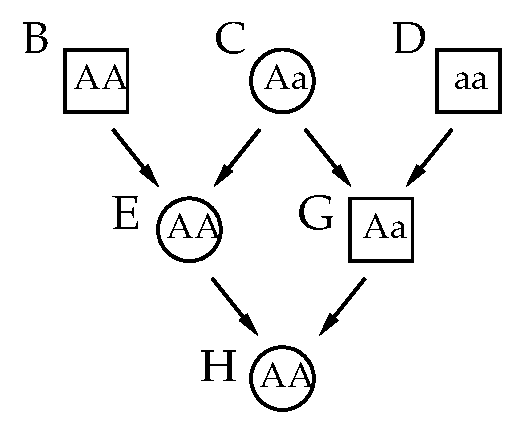
\includegraphics[width=2.5in]{fig5-2.ps}}

\end{slide}

\begin{slide}[Replace]{}

\centerline{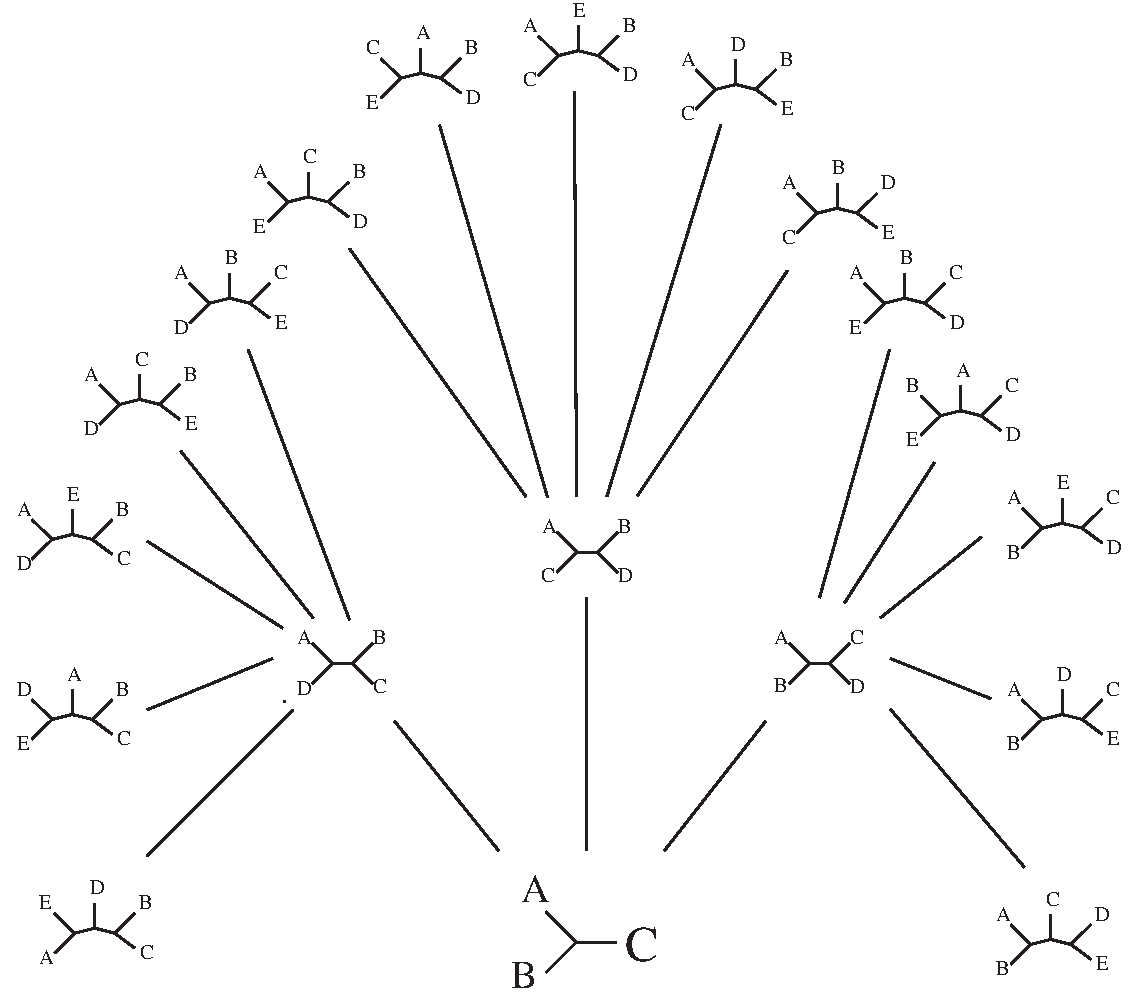
\includegraphics[width=2.0in]{fig5-3.ps}}

\end{slide}

\begin{slide}[Replace]{}

\centerline{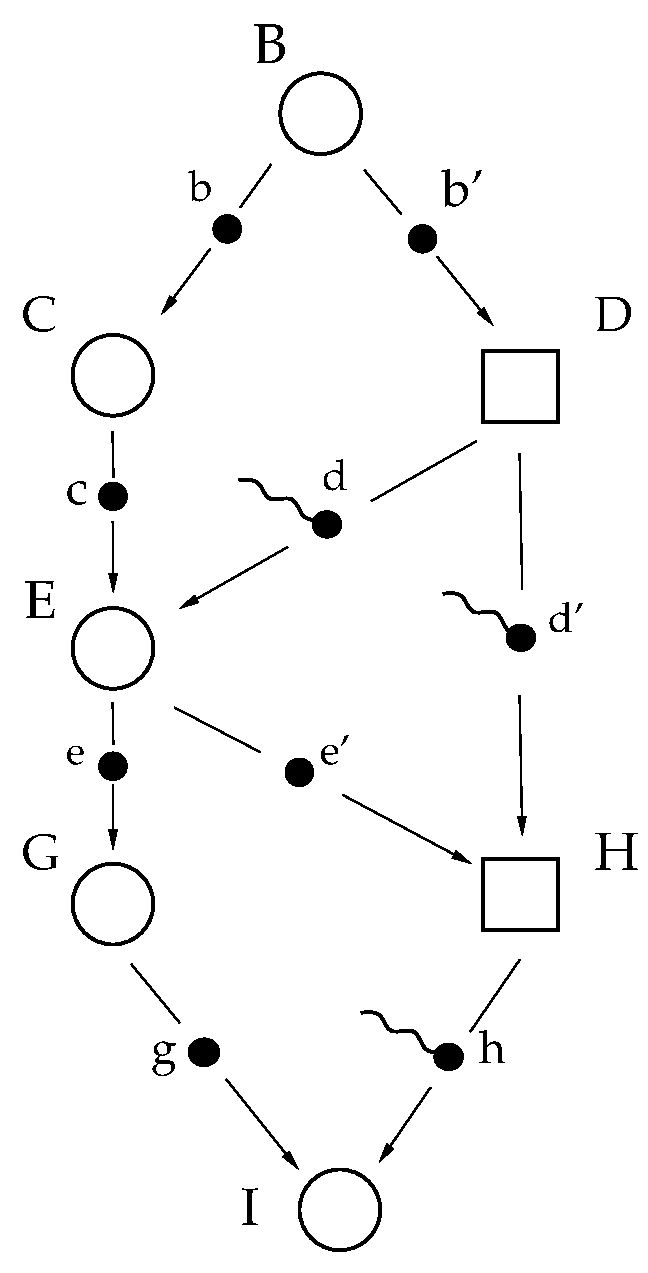
\includegraphics[width=1.3in]{fig5-4.ps}}

\end{slide}

\begin{slide}[Replace]{}

\centerline{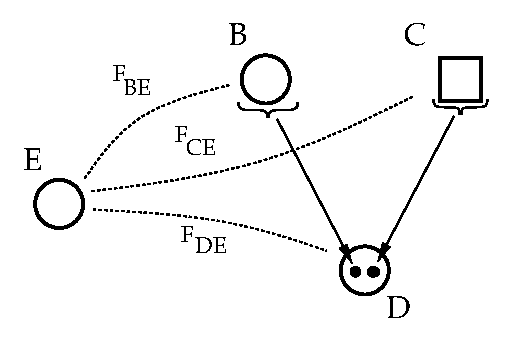
\includegraphics[width=2.5in]{fig5-5.ps}}

\end{slide}

\begin{slide}[Replace]{}

\centerline{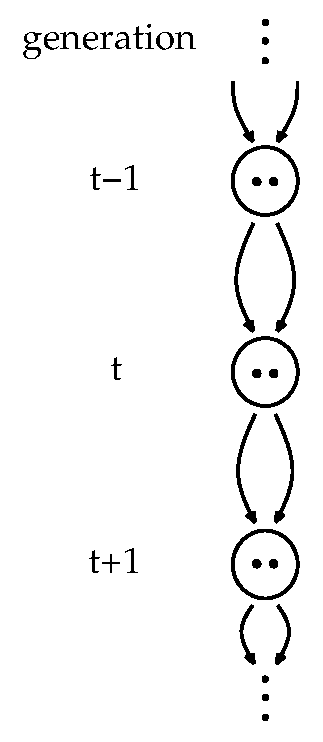
\includegraphics[width=1.0in]{fig5-6.ps}}

\end{slide}

\begin{slide}[Replace]{Reccurrent sib-mating}

\centerline{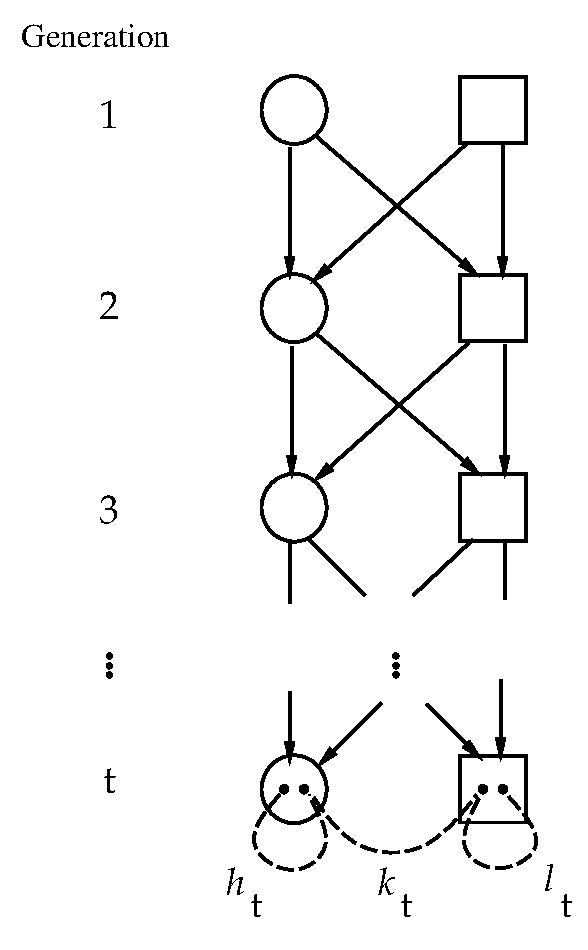
\includegraphics[width=1.8in]{fig5-7.ps}}

\end{slide}

\begin{slide}[Replace]{(non-)IBD from recurrent sib-mating}

\centerline{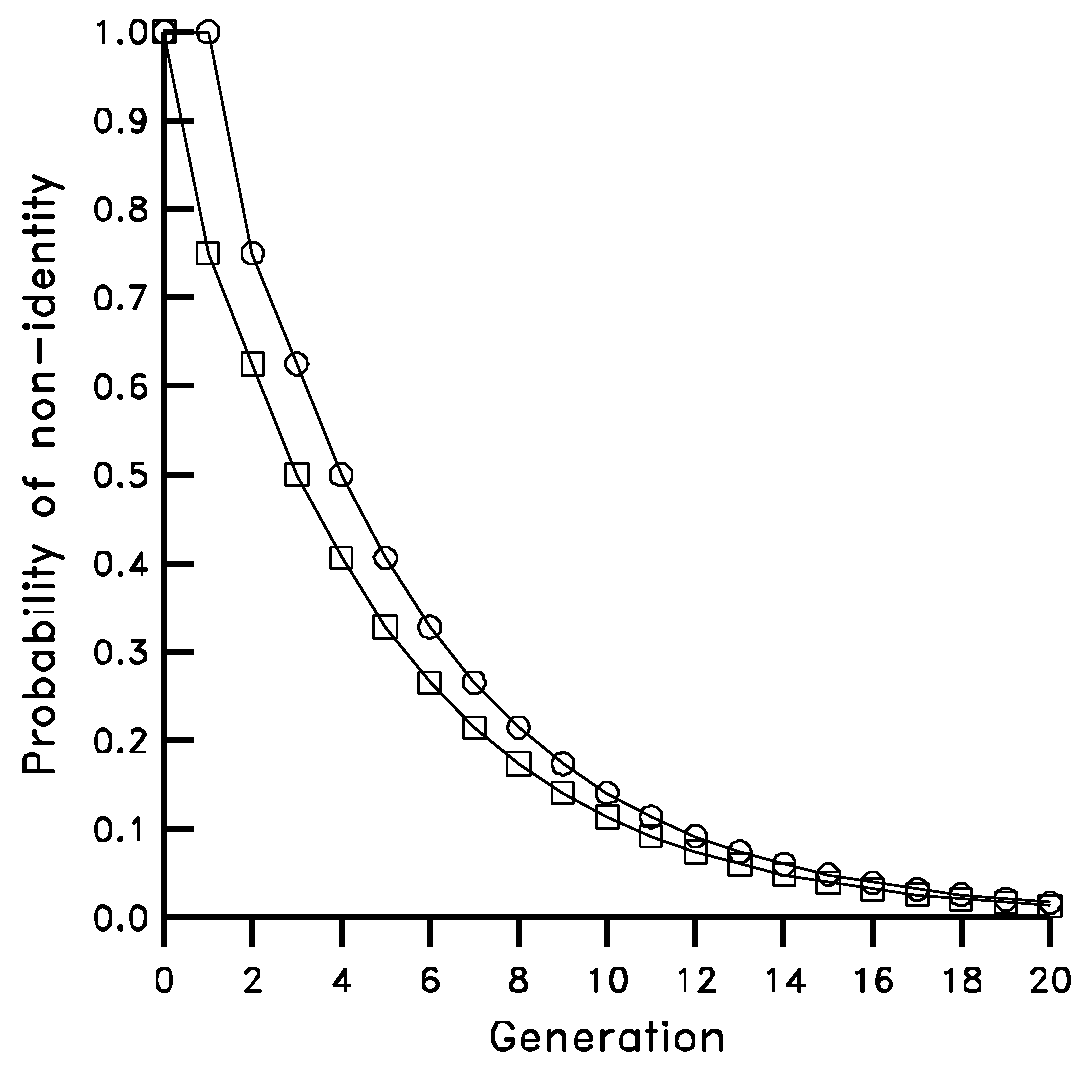
\includegraphics[width=2.5in]{fig5-8a.ps}}

\end{slide}

\begin{slide}[Replace]{On a log scale ... }

\centerline{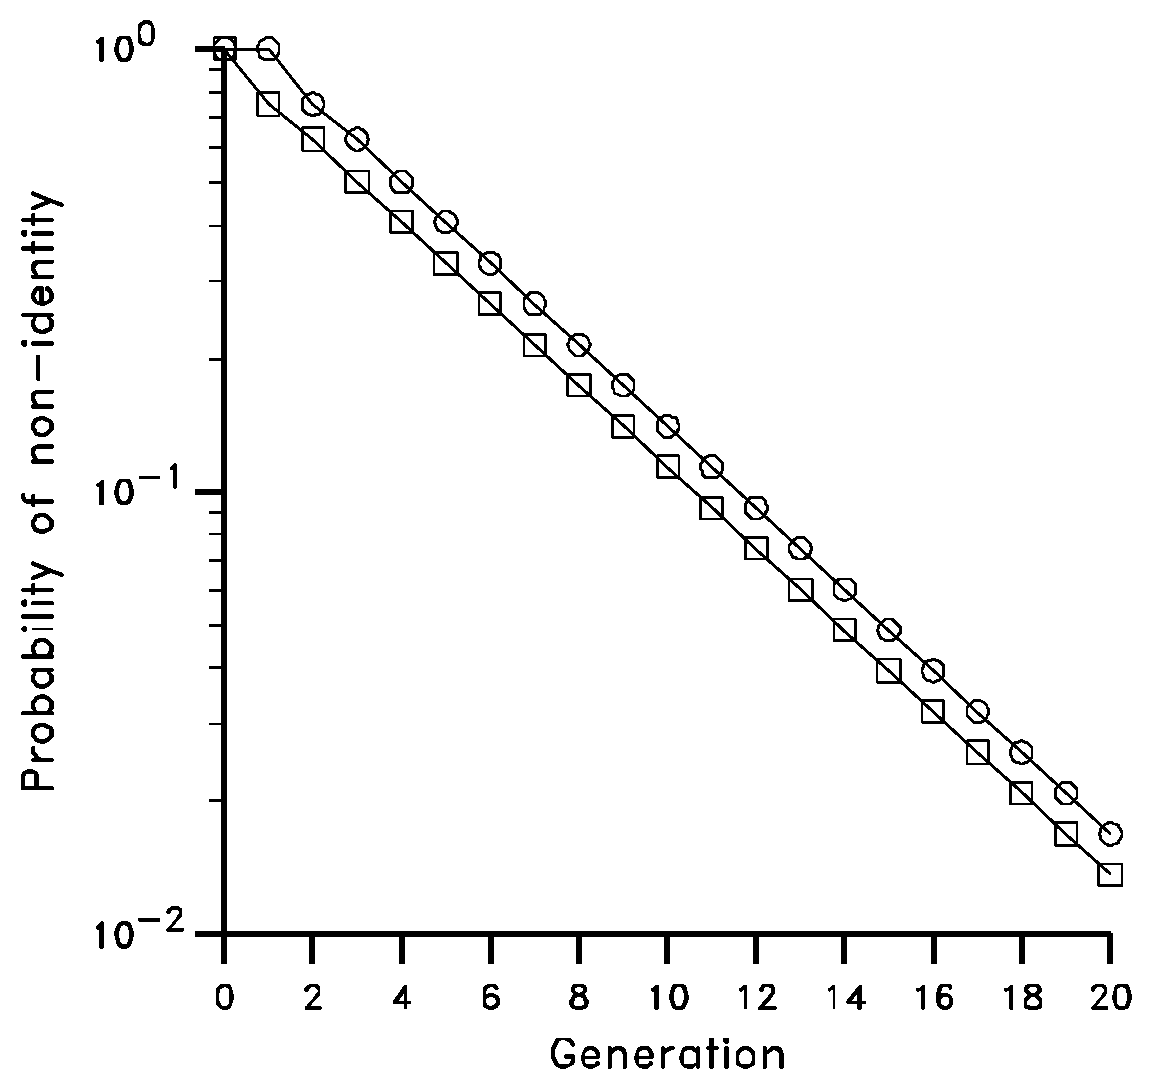
\includegraphics[width=2.5in]{fig5-9a.ps}}

\end{slide}

\begin{slide}[Replace]{East and Jones, 1918}

\begin{center}
\begin{tabular}{c c c}
\includegraphics[height=1.0in]{EdwardMEast.ps}  &
\includegraphics[height=1.5in]{DonaldFJones.ps} &
\includegraphics[height=1.5in]{EastJones1918.ps} \\
Edward M. East & Donald F. Jones & East and Jones, 1918\\
(1879-1938) & (1890-1963) &  
\end{tabular}
\end{center}

\end{slide}

\begin{slide}[Replace]{Inbreeding depression in {\it Drosophila} }
\vspace{-0.1in}

{\ptsize{8}
Table 1. Inbreeding depression (I.D.) in laboratory populations of Drosophila.
I.D. = 1-(zr/zo), where zo and zr are means of the random mating base, and the
completely inbred population (obtained by linear extrapolation), respectively.
Negative values imply an
increase in character value with inbreeding.}

{\ptsize{10}
\renewcommand\arraystretch{0.8}
\begin{tabular}{l l}
  Character                  &     I.D. (various studies)\\
\hline
  Competitive ability        &    0.84, 0.97\\
  Egg-to-adult viability     &    0.57, 0,44, 0.66*, 0.48*, 0.06\\
  Female fertility           &    0.81, 0.18, 0.35\\
  Female rate of reproduction&    0.81, 0.56, 0.96, 0.57\\
  Male mating ability        &    0.52*, 0.92, 0.76\\
  Male longevity             &    0.18*\\
  Male fertility             &    0.00*, 0.22*\\
  Male weight                &    0.07, 0.10\\
  Female weight              &    -0.10\\
  Abdominal bristle number   &    0.05, 0.06, 0.00\\
  Sternopleural bristle number &  -0.01, 0.00\\
  Wing length                  &  0.03, 0.01\\
  Thorax length                &  0.02\\
\end{tabular}

From Lynch, M. and J. B. Walsh. 1998. {\it Genetics and Analysis of
Quantitative Traits}. Sinauer Associates, Sunderland, Massachusetts.
}

\end{slide}

\begin{slide}[Replace]{Distribution of gene frequencies with genetic drift}

\centerline{\psfig{figure=fig6-1a.ps,width=1.6in}}
\centerline{\psfig{figure=fig6-1b.ps,width=1.6in}}
\centerline{\psfig{figure=fig6-1c.ps,width=1.6in}}

\noindent
{\ptsize{8}Distribution of gene frequencies (given as number of copies of the
{\it A} allele out of 20) among replicate populations in a diploid
Wright-Fisher model with $N = 10$ and initial frequency $p_0  =  0.3$ after
2 (top), 10 (middle), and 40 (bottom) generations.  Note that when almost all
populations are fixed
(T \ = \ 40) the remaining populations are distributed nearly uniformly over
the
unfixed classes.}

\end{slide}

\begin{slide}[Replace]{Change of heterozygosity and variance among lines}
\vspace{-0.1in}

\centerline{\psfig{figure=fig6-2.idraw,width=1.35in}}
\centerline{\psfig{figure=fig6-3.idraw,width=1.35in}}

\noindent
{\ptsize{8}Simulated genetic drift in 8 replicates of a diploid Wright-Fisher
model with $N = 10$ and $p_0  =  0.3$.  The upper graph shows the gene
frequencies in the eight replicate populations (lines) as well as the mean
gene frequency over those replicates (circles).  The lower graph shows
for the same simulation the
mean heterozygosity within replicates and the variance
of gene frequencies among replicates.}

\end{slide}

\end{document}

\end{document}

